\documentclass[]{article}
\usepackage{lmodern}
\usepackage{amssymb,amsmath}
\usepackage{ifxetex,ifluatex}
\usepackage{fixltx2e} % provides \textsubscript
\ifnum 0\ifxetex 1\fi\ifluatex 1\fi=0 % if pdftex
  \usepackage[T1]{fontenc}
  \usepackage[utf8]{inputenc}
\else % if luatex or xelatex
  \ifxetex
    \usepackage{mathspec}
    \usepackage{xltxtra,xunicode}
  \else
    \usepackage{fontspec}
  \fi
  \defaultfontfeatures{Mapping=tex-text,Scale=MatchLowercase}
  \newcommand{\euro}{€}
\fi
% use upquote if available, for straight quotes in verbatim environments
\IfFileExists{upquote.sty}{\usepackage{upquote}}{}
% use microtype if available
\IfFileExists{microtype.sty}{%
\usepackage{microtype}
\UseMicrotypeSet[protrusion]{basicmath} % disable protrusion for tt fonts
}{}
\usepackage[margin=1in]{geometry}
\usepackage{longtable,booktabs}
\usepackage{graphicx}
\makeatletter
\def\maxwidth{\ifdim\Gin@nat@width>\linewidth\linewidth\else\Gin@nat@width\fi}
\def\maxheight{\ifdim\Gin@nat@height>\textheight\textheight\else\Gin@nat@height\fi}
\makeatother
% Scale images if necessary, so that they will not overflow the page
% margins by default, and it is still possible to overwrite the defaults
% using explicit options in \includegraphics[width, height, ...]{}
\setkeys{Gin}{width=\maxwidth,height=\maxheight,keepaspectratio}
\ifxetex
  \usepackage[setpagesize=false, % page size defined by xetex
              unicode=false, % unicode breaks when used with xetex
              xetex]{hyperref}
\else
  \usepackage[unicode=true]{hyperref}
\fi
\hypersetup{breaklinks=true,
            bookmarks=true,
            pdfauthor={},
            pdftitle={The Mathematics of Enigma},
            colorlinks=true,
            citecolor=blue,
            urlcolor=blue,
            linkcolor=magenta,
            pdfborder={0 0 0}}
\urlstyle{same}  % don't use monospace font for urls
\setlength{\parindent}{0pt}
\setlength{\parskip}{6pt plus 2pt minus 1pt}
\setlength{\emergencystretch}{3em}  % prevent overfull lines
\setcounter{secnumdepth}{0}

%%% Use protect on footnotes to avoid problems with footnotes in titles
\let\rmarkdownfootnote\footnote%
\def\footnote{\protect\rmarkdownfootnote}

%%% Change title format to be more compact
\usepackage{titling}

% Create subtitle command for use in maketitle
\newcommand{\subtitle}[1]{
  \posttitle{
    \begin{center}\large#1\end{center}
    }
}

\setlength{\droptitle}{-2em}

  \title{The Mathematics of Enigma}
    \pretitle{\vspace{\droptitle}\centering\huge}
  \posttitle{\par}
    \author{}
    \preauthor{}\postauthor{}
    \date{}
    \predate{}\postdate{}
  

\begin{document}

\maketitle


\begin{figure}[htbp]
\centering
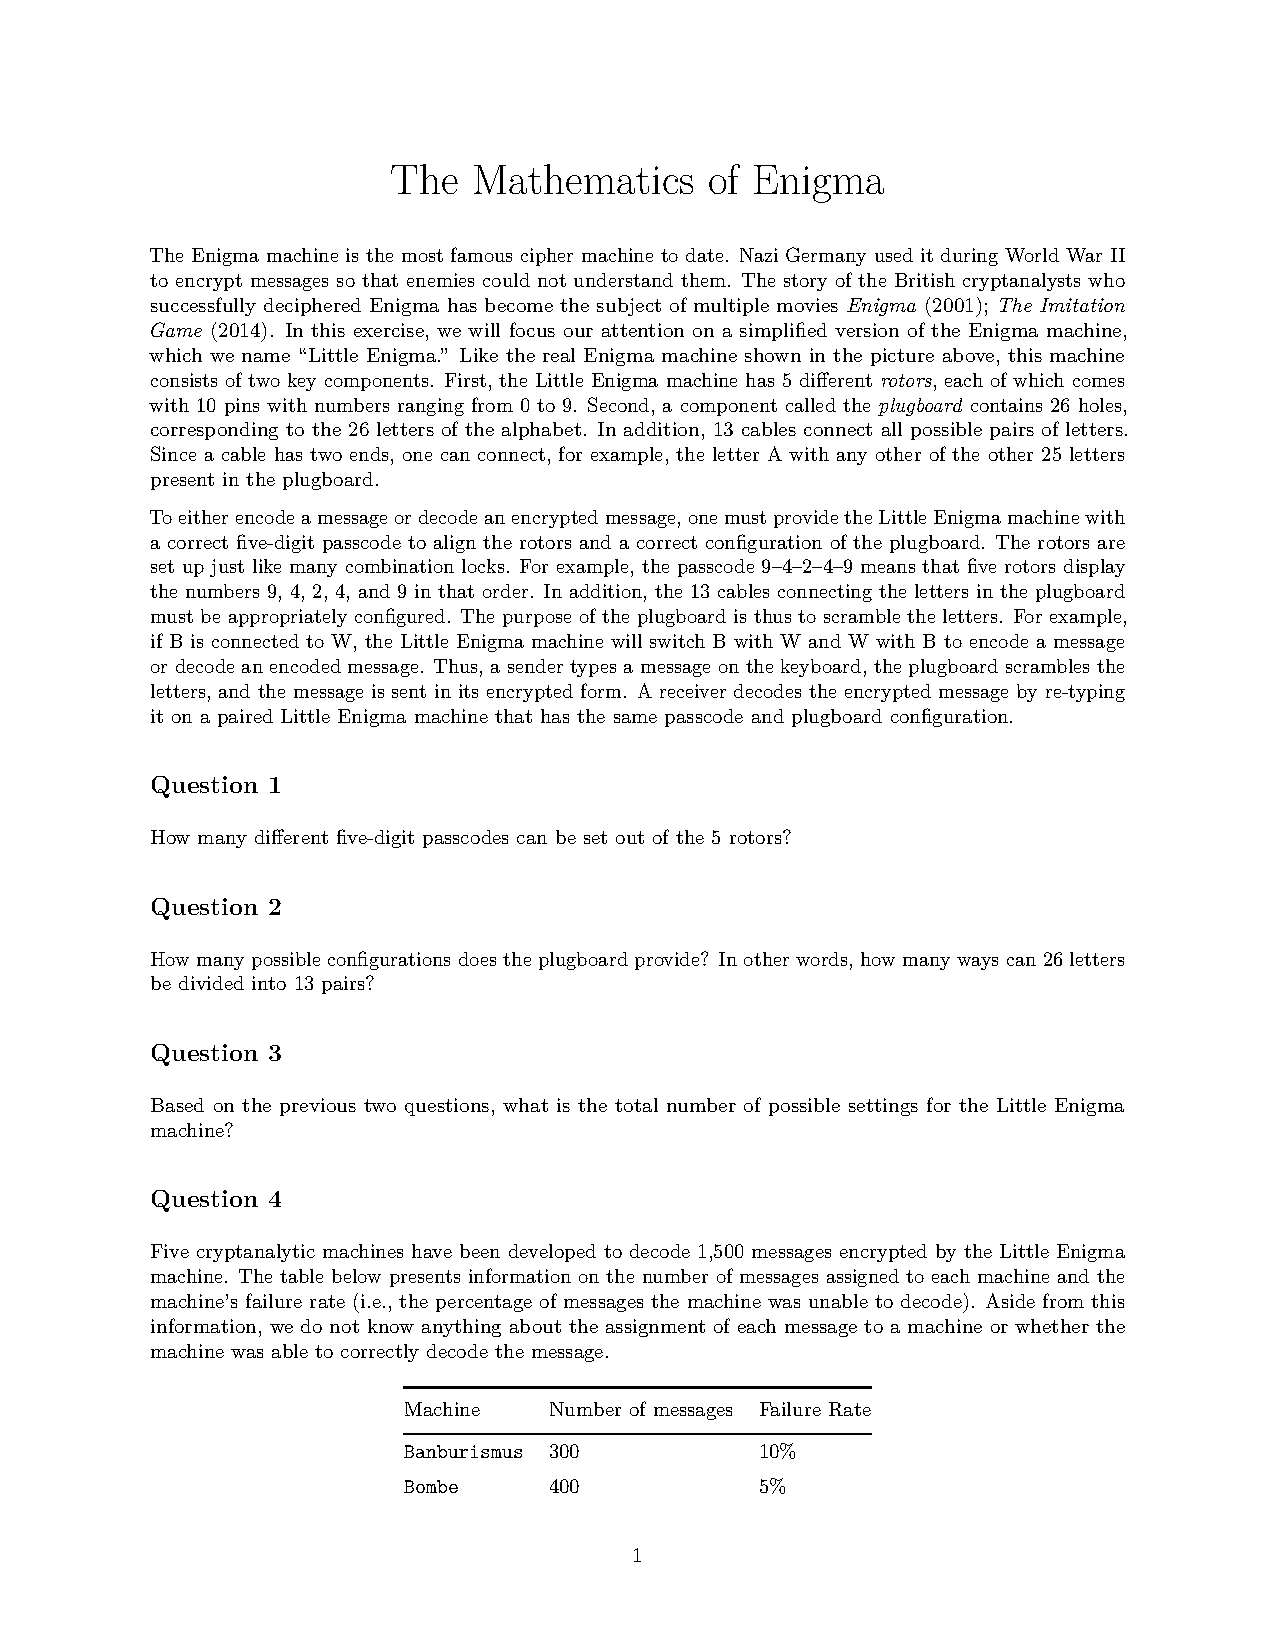
\includegraphics{pics/enigma.jpg}
\caption{The Enigma Machine}
\end{figure}

The Enigma machine is the most famous cipher machine to date. Nazi
Germany used it during World War II to encrypt messages so that enemies
could not understand them. The story of the British cryptanalysts who
successfully deciphered Enigma has become the subject of multiple movies
\emph{Enigma} (2001); \emph{The Imitation Game} (2014). In this
exercise, we will focus our attention on a simplified version of the
Enigma machine, which we name ``Little Enigma.'' Like the real Enigma
machine shown in the picture above, this machine consists of two key
components. First, the Little Enigma machine has 5 different
\emph{rotors}, each of which comes with 10 pins with numbers ranging
from 0 to 9. Second, a component called the \emph{plugboard} contains 26
holes, corresponding to the 26 letters of the alphabet. In addition, 13
cables connect all possible pairs of letters. Since a cable has two
ends, one can connect, for example, the letter A with any other of the
other 25 letters present in the plugboard.

To either encode a message or decode an encrypted message, one must
provide the Little Enigma machine with a correct five-digit passcode to
align the rotors and a correct configuration of the plugboard. The
rotors are set up just like many combination locks. For example, the
passcode 9--4--2--4--9 means that five rotors display the numbers 9, 4,
2, 4, and 9 in that order. In addition, the 13 cables connecting the
letters in the plugboard must be appropriately configured. The purpose
of the plugboard is thus to scramble the letters. For example, if B is
connected to W, the Little Enigma machine will switch B with W and W
with B to encode a message or decode an encoded message. Thus, a sender
types a message on the keyboard, the plugboard scrambles the letters,
and the message is sent in its encrypted form. A receiver decodes the
encrypted message by re-typing it on a paired Little Enigma machine that
has the same passcode and plugboard configuration.

\subsection{Question 1}\label{question-1}

How many different five-digit passcodes can be set out of the 5 rotors?

\subsection{Question 2}\label{question-2}

How many possible configurations does the plugboard provide? In other
words, how many ways can 26 letters be divided into 13 pairs?

\subsection{Question 3}\label{question-3}

Based on the previous two questions, what is the total number of
possible settings for the Little Enigma machine?

\subsection{Question 4}\label{question-4}

Five cryptanalytic machines have been developed to decode 1,500 messages
encrypted by the Little Enigma machine. The table below presents
information on the number of messages assigned to each machine and the
machine's failure rate (i.e., the percentage of messages the machine was
unable to decode). Aside from this information, we do not know anything
about the assignment of each message to a machine or whether the machine
was able to correctly decode the message.

\begin{longtable}[c]{@{}lll@{}}
\toprule\addlinespace
Machine & Number of messages & Failure Rate
\\\addlinespace
\midrule\endhead
\texttt{Banburismus} & 300 & 10\%
\\\addlinespace
\texttt{Bombe} & 400 & 5\%
\\\addlinespace
\texttt{Herivel} & 250 & 15\%
\\\addlinespace
\texttt{Crib} & 340 & 17\%
\\\addlinespace
\texttt{Hut 6} & 210 & 20\%
\\\addlinespace
\bottomrule
\end{longtable}

Suppose that we select one message at random from the pool of all 1,500
messages but found out this message was not properly decoded. Which
machine is most likely responsible for this mistake?

\subsection{Question 5}\label{question-5}

Write an R function that randomly configures the plugboard. This
function will take no input but randomly selects a set of 13 pairs of
letters. The output object should be a $2 \times 13$ matrix for which
each column represents a pair of letters. You may use the built-in R
object \texttt{letters}, which contains the 26 letters of the alphabet
as a character vector. Name the function \texttt{plugboard}.

\subsection{Question 6}\label{question-6}

Write an R function that encodes and decodes a message given a plugboard
configuration set by the \texttt{plugboard} function from the previous
question. This function should take the output of the \texttt{plugboard}
function as well as a message to be encoded (decoded) as inputs, and
return an encoded (decoded) message. You may wish to use the
\texttt{gsub} function, which replaces a pattern in a character string
with another specified pattern. The \texttt{tolower} function, which
makes characters in a character vector lowercase, and \texttt{toupper}
function, which capitalizes characters in a character vector, can also
help.

\end{document}
